%; whizzy paragraph -pdf xpdf -latex ./whizzypdfptex.sh
%; whizzy-paragraph "^\\\\begin{frame}\\|\\\\emtext"
% latex beamer presentation.
% platex, latex-beamer でコンパイルすることを想定。 

%     Tokyo Debian Meeting resources
%     Copyright (C) 2012 Junichi Uekawa

%     This program is free software; you can redistribute it and/or modify
%     it under the terms of the GNU General Public License as published by
%     the Free Software Foundation; either version 2 of the License, or
%     (at your option) any later version.

%     This program is distributed in the hope that it will be useful,
%     but WITHOUT ANY WARRANTY; without even the implied warreanty of
%     MERCHANTABILITY or FITNESS FOR A PARTICULAR PURPOSE.  See the
%     GNU General Public License for more details.

%     You should have received a copy of the GNU General Public License
%     along with this program; if not, write to the Free Software
%     Foundation, Inc., 51 Franklin St, Fifth Floor, Boston, MA  02110-1301 USA

\documentclass[cjk,dvipdfmx,12pt]{beamer}
\usetheme{Tokyo}
\usepackage{monthlypresentation}

%  preview (shell-command (concat "evince " (replace-regexp-in-string "tex$" "pdf"(buffer-file-name)) "&")) 
%  presentation (shell-command (concat "xpdf -fullscreen " (replace-regexp-in-string "tex$" "pdf"(buffer-file-name)) "&"))
%  presentation (shell-command (concat "evince " (replace-regexp-in-string "tex$" "pdf"(buffer-file-name)) "&"))

%http://www.naney.org/diki/dk/hyperref.html
%日本語EUC系環境の時
\AtBeginDvi{\special{pdf:tounicode EUC-UCS2}}
%シフトJIS系環境の時
%\AtBeginDvi{\special{pdf:tounicode 90ms-RKSJ-UCS2}}

\newenvironment{commandlinesmall}%
{\VerbatimEnvironment
  \begin{Sbox}\begin{minipage}{1.0\hsize}\begin{fontsize}{8}{8} \begin{BVerbatim}}%
{\end{BVerbatim}\end{fontsize}\end{minipage}\end{Sbox}
  \setlength{\fboxsep}{8pt}
% start on a new paragraph

\vspace{6pt}% skip before
\fcolorbox{dancerdarkblue}{dancerlightblue}{\TheSbox}

\vspace{6pt}% skip after
}
%end of commandlinesmall

\title{東京エリアDebian勉強会}
\subtitle{第134回 2015年12月度}
\author{野島貴英}
\date{2015年12月19日}
\logo{
\includegraphics[width=8cm]{image200607/openlogo-light.eps}}

\begin{document}

\begin{frame}
\titlepage{}
\end{frame}

\begin{frame}{Agenda}
 \begin{minipage}[t]{0.45\hsize}
  \begin{itemize}
   \item 事前課題発表
   \item 最近あったDebian関連のイベント報告
	 \begin{itemize}
	 \item 第133回東京エリアDebian勉強会
	 \end{itemize}
  \end{itemize}
 \end{minipage} 
 \begin{minipage}[t]{0.45\hsize}
  \begin{itemize}
   \item Debian Trivia Quiz
   \item Debian おすすめのパッケージを参加者に聞いてみた
   \item Debian モバイル wifi ルータ化
   \item 今日の宴会場所
  \end{itemize}
 \end{minipage}
\end{frame}

\section{事前課題}
\emtext{事前課題}
{\footnotesize
 \begin{prework}{ henrich }
  \begin{enumerate}
  \item Q.hack time に何をしますか?\\
    A. バグレポートを読んで、直せそうなところを整理します。
  \end{enumerate}
\end{prework}

\begin{prework}{ wskoka }
  \begin{enumerate}
  \item Q.hack time に何をしますか?\\
    A. tilegxのdebian化
  \end{enumerate}
\end{prework}

\begin{prework}{ rosh }
  \begin{enumerate}
  \item Q.hack time に何をしますか?\\
    A. 自分の担当するパッケージをメインテインする (wide-dhcpv6とadjtimex)
  \end{enumerate}
\end{prework}

\begin{prework}{ tai }
  \begin{enumerate}
  \item Q.hack time に何をしますか?\\
    A. もくもくとパッケージングリハビリとbugs.d.oの落穂ひろいをします。
  \end{enumerate}
\end{prework}

\begin{prework}{ koedoyoshida }
  \begin{enumerate}
  \item Q.hack time に何をしますか?\\
    A. 予定は未定
  \end{enumerate}
\end{prework}

\begin{prework}{ dictoss }
  \begin{enumerate}
  \item Q.hack time に何をしますか?\\
    A. kfreebsd関連作業
  \end{enumerate}
\end{prework}

\begin{prework}{ nametake }
  \begin{enumerate}
  \item Q.hack time に何をしますか?\\
    A. windowsタブレットにdebianインストール
  \end{enumerate}
\end{prework}

\begin{prework}{ yy\_y\_ja\_jp }
  \begin{enumerate}
  \item Q.hack time に何をしますか?\\
    A. DDTSS
  \end{enumerate}
\end{prework}

\begin{prework}{ かじ }
  \begin{enumerate}
  \item Q.hack time に何をしますか?\\
    A. 前回参加できなかったので、今回はwaylandで簡単なサンプルを作ってみたい。\\
参考にしたいのは\\
http://d.hatena.ne.jp/devm33/20140414/1397473785
  \end{enumerate}
\end{prework}

\begin{prework}{ 野島 }
  \begin{enumerate}
  \item Q.hack time に何をしますか?\\
    A. DDTSSとか
  \end{enumerate}
\end{prework}




}

\section{イベント報告}
\emtext{イベント報告}

\begin{frame}{第133回東京エリアDebian勉強会 }

\begin{itemize}
\item 場所はdotsさんをお借りしての開催でした。
\item 参加者は9名でした。
\item セミナ内容は杉本さんによる「Debian GNU/kFreeBSD セットアップガイド 2015 年版」でした。
\item 残りの時間でhack timeを行い、成果発表をしました。
\end{itemize} 
\end{frame}

\begin{frame}{第133回東京エリアDebian勉強会(つづき)}

 「Debian GNU/kFreeBSD セットアップガイド 2015 年版」は、kFreeBSDのセットアップについて最近のやり方についての発表でした。昨今、検索エンジンで検索できるkFreeBSDのセットアップ方法について内容が古いものが多いとのことです。本発表の資料で今時のやり方にアップデートが行われる(少なくとも検索上位になる)と良いですね。
\end{frame}

\begin{frame}{第133回東京エリアDebian勉強会(つづき)}

  また、発表後のhack time中に、
\begin{center}
\LARGE
  kFreeBSDを一般のIaaS型クラウドサービスへ直接インストールに成功した
\end{center}
強者が現れるなど、面白い展開をしていました。

\end{frame}

\if0
\section{Debian Trivia Quiz}
\emtext{Debian Trivia Quiz}
\begin{frame}{Debian Trivia Quiz}

  Debian の常識、もちろん知ってますよね?
知らないなんて恥ずかしくて、知らないとは言えないあんなことやこんなこと、
みんなで確認してみましょう。

今回の出題範囲は\url{debian-devel-announce@lists.debian.org},
\url{debian-news@lists.debian.org} に投稿された
内容などからです。

\end{frame}

\subsection{問題}

%; whizzy-master ../debianmeetingresume201311.tex
% $B0J>e$N@_Dj$r$7$F$$$k$?$a!"$3$N%U%!%$%k$G(B M-x whizzytex $B$9$k$H!"(Bwhizzytex$B$,MxMQ$G$-$^$9!#(B
%

\santaku
{2015/10/22$B$N(BDPN$B$N%a!<%k$+$iDj4|E*$K$J$,$l$F$$$?$$$/$D$+$N%H%T%C%/$,(BWeb$B$N$_$K7G<($5$l$k$h$&$K$J$j$^$7$?!#$I$3$K7G<($5$l$k!)(B}
{http://www.debian.or.jp/}
{http://www.debian.org/}
{http://bits.debian.org/}
{C}
{2015/10/22$B$N(BDPN$B$N%a!<%k$+$i!"=>MhN.$l$F$$$?(BDPN$B$N%a!<%k$N9=@.$,:~?7$5$l$^$7$?!#$3$A$i$KH<$$!"%;%-%e%j%F%#$K$D$$$F$N%"%J%&%s%9$H!"?7$7$$(BDD/DM$B$N%"%J%&%s%9$O!"(BDPN$B$N%a!<%k$K$O4^$^$l$:!"(BWeb$B%Z!<%8$K7G:\$5$l$k$N$_$H$J$j$^$7$?!#(B}

\santaku
{2015/11/7$B$K$F!"$H$"$k%$%s%9%?%s%H%a%C%;%s%8%c!<MQ%W%m%H%3%k$N%5!<%S%9$,A4(BDebian Developer$B$G;H$($k$h$&$K$J$C$?$H$N%"%J%&%s%9$,$"$j$^$7$?!#%W%m%H%3%k$NL>A0$O<!$N$I$l!)(B}
{XMPP}
{IRC}
{IP Messanger}
{A}
{XMPP$B$O%*!<%W%s$J%$%s%9%?%s%H%a%C%;%s%8%c!<MQ%W%m%H%3%k$N#1$D!#$J$*!"(BDebian$B4X78<T$NMxMQ$K$"$?$C$F>\$7$/$O!"(Bhttp://rtc.debian.org$B$r;2>H!#(B}

\santaku
{2015/10/30$B$K$F!"(BDebian$B$K$F!"(B2$B2sL\$N8xJg$,9T$o$l$?Lr$^$o$j$O<!$N$I$l!)(B}
{2016 DPN}
{technical commitee}
{2016 Debian JP$B2qD9(B}
{B}
{2$BL>$[$I!"(BDebian Developer$B$NJ}$G(Btechnical comittee$B$G3hLv$G$-$kJ}Jg=8$H$N$3$H$G$9!#8=?&(Btechnical comittee$B$N?M$i$,!"(B2015/12/31$B$GG$4|$,@Z$l$F$7$^$&$H$$$&$3$H$G!"$=$l$^$G$K8uJd<T$r5s$2$kI,MW$,$"$k$H$N$3$H$G$9!#(B}



\fi

\section{Debian おすすめのパッケージを参加者に聞いてみた}
\emtext{Debian おすすめのパッケージを参加者に聞いてみた}

\begin{frame}{はじめに}

  前回の東京エリアDebian勉強会で、「参加者にDebianのおすすめパッケージを聞いてみたらおもしろいんじゃない?」という企画案がでました。今回、東京エリアDebian勉強会の参加登録時のアンケートを利用して聞いてみました。

\end{frame}

\begin{frame}{screenfetch パッケージ}

  \begin{description}
    \item [推薦者] henrichさん
   \item [コメント] cowsayみたいなちょっとユーモラスなパッケージです。
  \end{description}

\end{frame}

\begin{frame}{screenfetch パッケージ(つづき)}

\begin{figure}[htbp]
\begin{tabular}{cc}
\begin{minipage}{0.5\hsize}
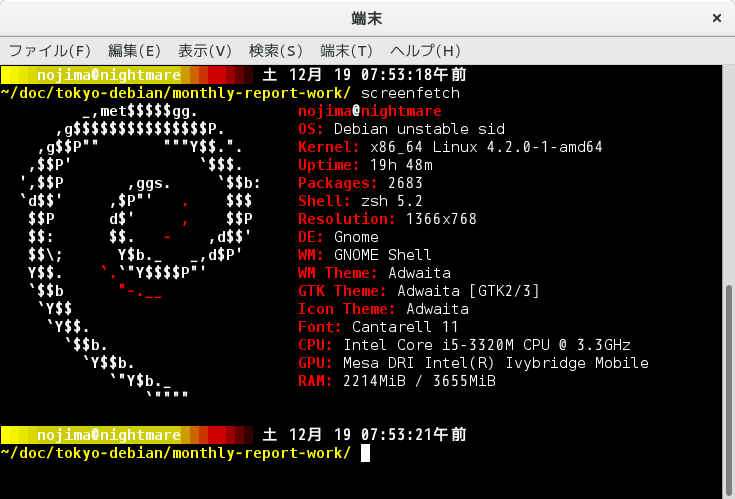
\includegraphics[width=0.8\hsize]{image201512/debian-screenfetch.png}
\caption{screenfetch起動}
\end{minipage}
\begin{minipage}{0.5\hsize}
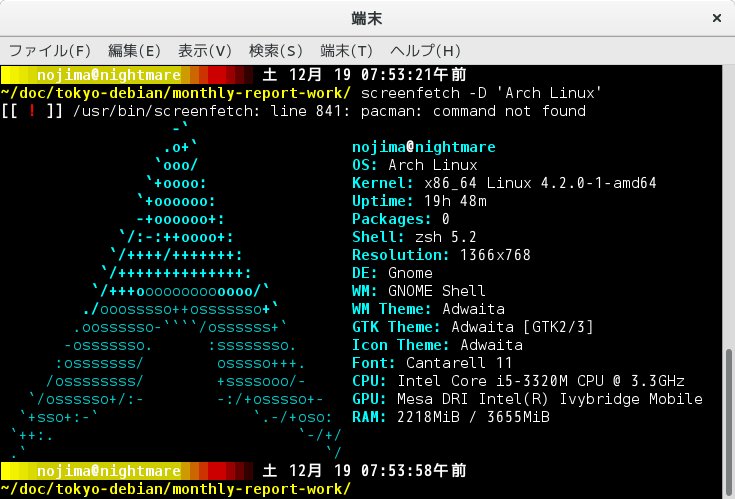
\includegraphics[width=0.8\hsize]{image201512/arch-screenfetch.png}
\caption{-D 'Arch Linux'の場合}
\end{minipage}
\end{tabular}
\end{figure}

\end{frame}

\begin{frame}{screenfetch パッケージ(つづき)}

\begin{figure}[htbp]
\begin{tabular}{cc}
\begin{minipage}{0.5\hsize}
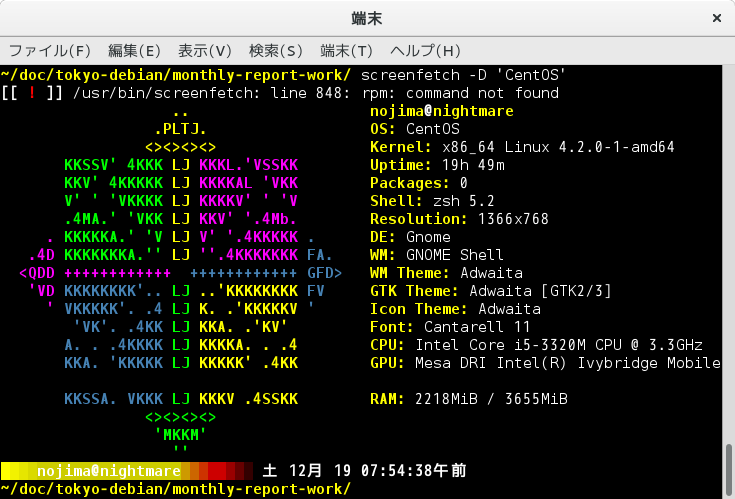
\includegraphics[width=0.8\hsize]{image201512/centos-screenfetch.png}
\caption{-D 'CentOS'の場合}
\end{minipage}
\begin{minipage}{0.5\hsize}
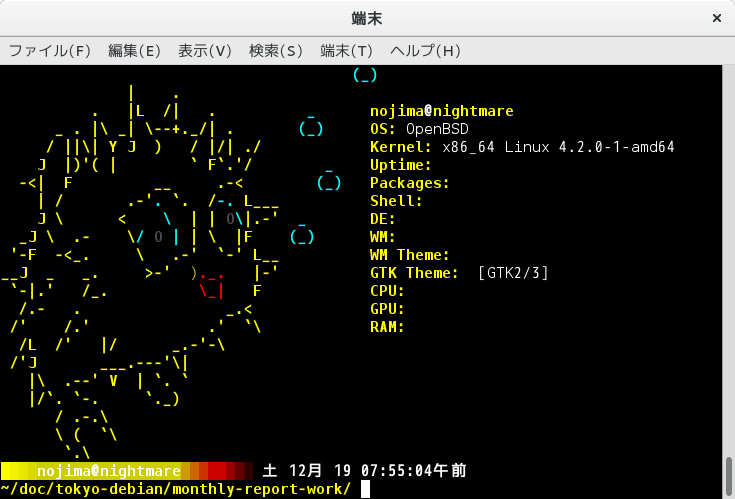
\includegraphics[width=0.8\hsize]{image201512/openbsd-screenfetch.png}
\caption{-D 'OpenBSD'の場合}
\end{minipage}
\end{tabular}
\end{figure}

\end{frame}

\begin{frame}{adjtimex パッケージ}

  \begin{description}
    \item [推薦者] roshさん
   \item [コメント] 自分がメンテする adjtimex をお勧めいたします。adjtimex パッケージに adjtimexconfig コマンドを実行すれば、70秒をかけて、kernel に時間に関する tick と frequency のお勧め値が計算し、/etc/default/ajdtimex に保存されます。再起動の際に、その値が kernel に設定されます。NTP client と違って、バックグランド service がありません。起動時に kernel パラメータを設定することで、システム時間がある程度早く・遅くにならないように、精度を向上できます。
  \end{description}

\end{frame}

\begin{frame}{fpm}
  \begin{description}
    \item [推薦者] taiさん
   \item [コメント] パッケージというよりパッケージビルダーfpmがお気に入りです。
aufsやunionfsとくっつけて、chroot ... sh -c './configure \&\& make' \&\& fpm ... /unionfs/cow-dirで手抜きdebやrpmを量産していました。なぜfpmはDebian package化されていないのだろう?
  \end{description}

\end{frame}

\begin{frame}{geeqie パッケージ}

  \begin{description}
    \item [推薦者] dictossさん
   \item [コメント] 画像ビューア。快適に動きます。
  \end{description}

\end{frame}

\begin{frame}{geeqie パッケージ(つづき)}

\begin{figure}[htbp]
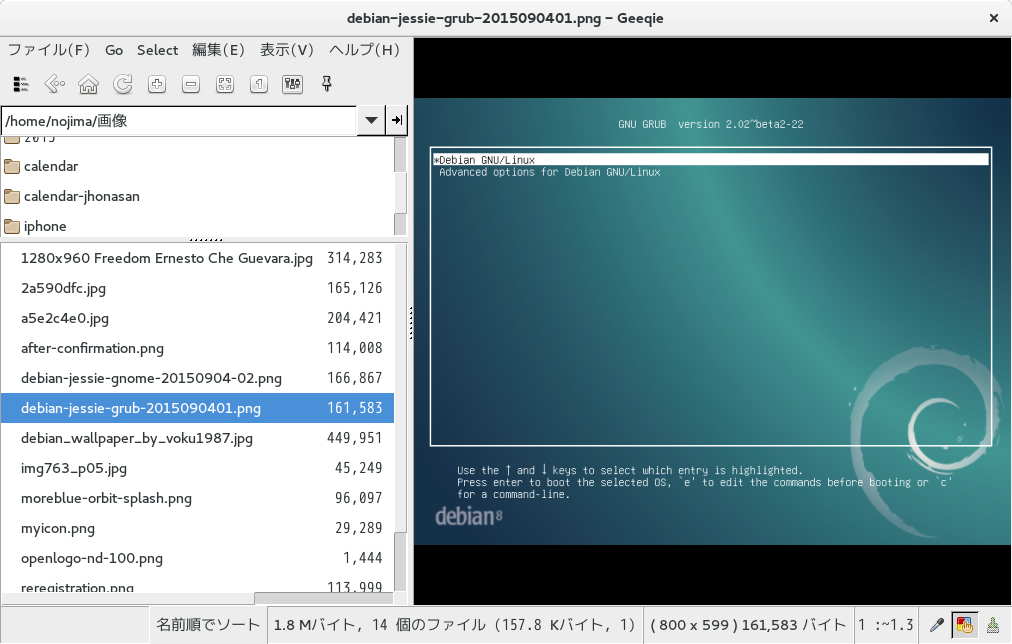
\includegraphics[width=0.8\hsize]{image201512/geeqie.png}
\caption{geeqieの様子}
\end{figure}

\end{frame}

\begin{frame}{openvpn パッケージ}

  \begin{description}
    \item [推薦者] dictossさん
   \item [コメント] 自宅へ接続するときに便利です。
  \end{description}

\end{frame}

\begin{frame}{python-dateutil パッケージ}

  \begin{description}
    \item [推薦者] dictossさん
   \item [コメント] ISO 8601形式の日時文字列から日時オブジェクトへ変換するのに便利なライブラリです。
  \end{description}

\end{frame}

\begin{frame}{apache2 パッケージ}

  \begin{description}
    \item [推薦者] nametake
   \item [コメント] 構成に独特のこだわりを感じる
  \end{description}

\end{frame}

\begin{frame}{popularity-contest パッケージ}

  \begin{description}
    \item [推薦者] yy\_y\_ja\_jp
   \item [コメント] 自動でお勧めしましょう
  \end{description}

\end{frame}

\begin{frame}{wavemon パッケージ}

  \begin{description}
    \item [推薦者] かじ
   \item [コメント] wavemonの表示がかっこいい。
  \end{description}

\end{frame}

\begin{frame}{wavemon パッケージ(つづき)}

\begin{figure}[htbp]
\begin{tabular}{cc}
\begin{minipage}{0.5\hsize}
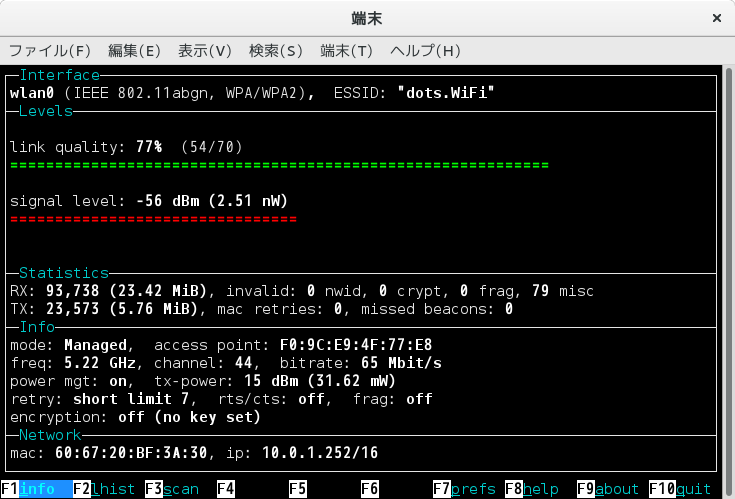
\includegraphics[width=0.8\hsize]{image201512/wavemon-1.png}
\caption{起動後の画面}
\end{minipage}
\begin{minipage}{0.5\hsize}
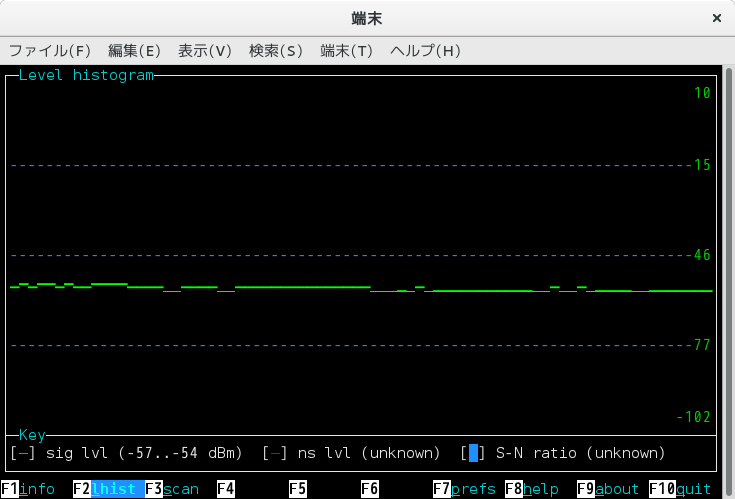
\includegraphics[width=0.8\hsize]{image201512/wavemon-2.png}
\caption{hlistの画面}
\end{minipage}
\end{tabular}
\end{figure}
\end{frame}

\begin{frame}{wavemon パッケージ(つづき)}

\begin{figure}[htbp]
\begin{tabular}{cc}
\begin{minipage}{0.5\hsize}
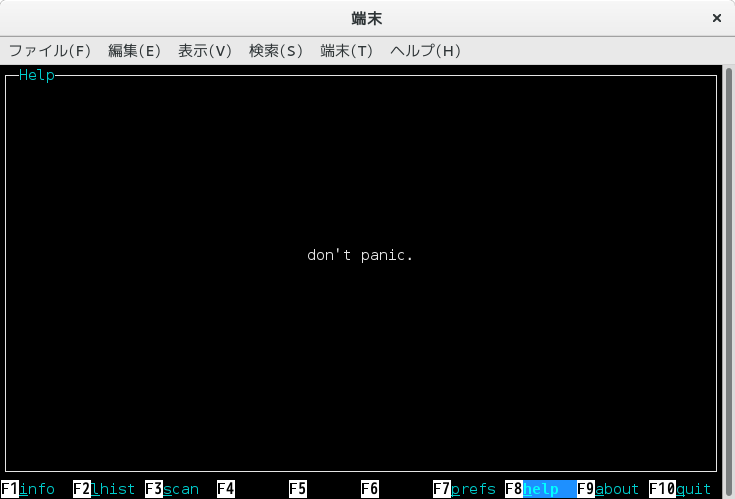
\includegraphics[width=0.8\hsize]{image201512/wavemon-3.png}
\caption{helpの画面}
\end{minipage}
\begin{minipage}{0.5\hsize}
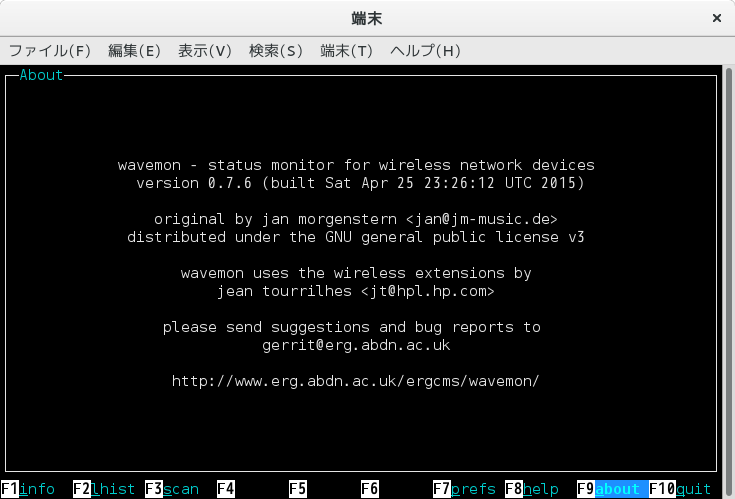
\includegraphics[width=0.8\hsize]{image201512/wavemon-4.png}
\caption{aboutの画面(動画でお見せできないのが残念)}
\end{minipage}
\end{tabular}
\end{figure}
\end{frame}

\begin{frame}{dnsmasq パッケージ}

  \begin{description}
    \item [推薦者] 野島
   \item [コメント] これ一本だけで、DHCPサーバ、PXEサーバ、簡易DNSサーバを、少ない設定量であっと言う間に作れる。設定項目も多すぎず少なすぎずの絶妙な設計であり、使い捨ての環境を作るのにとても便利。参考:第109回東京エリアDebian勉強会「Debian で dnsmasq を使う」http://tokyodebian.alioth.debian.org/2014-02.html
  \end{description}

\end{frame}

\begin{frame}{kvm パッケージ}

  \begin{description}
    \item [推薦者] 野島
   \item [コメント] コマンドラインにちょこちょこっとLiveイメージのisoとともに指定して起動するだけで、仮想環境で様々なOSを試せる。例:Android-x86のLiveデモ起動:kvm -m 2G -soundhw es1370 -net nic -net user -cdrom ./android-x86-5.1-rc1.iso
  \end{description}

\end{frame}

\begin{frame}{kvm パッケージ(つづき)}

\begin{figure}[htbp]
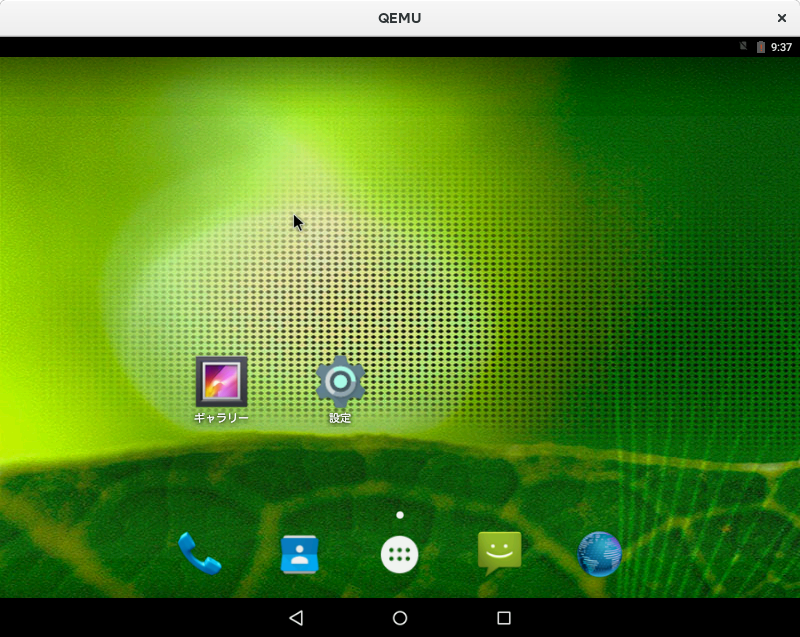
\includegraphics[width=0.8\hsize]{image201512/kvm.png}
\caption{kvmでAndroid-x86 Live CDを起動}
\end{figure}
  
\end{frame}

\begin{frame}{おわりに}

 もっといろいろ素敵なパッケージがありましたら、随時おしえてくださいませ。
  
\end{frame}

\section{Debian モバイル wifi ルータ化}
\emtext{Debian モバイル wifi ルータ化}

\begin{frame}{はじめに}

 最近のモバイルルータは、7GBytes/月、300MBytes/日などの、一定の通信量を超えるとたちまち通信制限がかかってしまい、とても実用にならないぐらいに通信帯域を絞られてしまいます。
  
 たまたま、手元に通信制限が非常にゆるい(というか気にならない)FOMAのモデムがありましたので、こちらとDebianを使ってモバイルルータが作れないかを試してみました。また、Linuxで無線APを作る時の仕組みについてもちょっと調べてみました。
 
\end{frame}

\begin{frame}{用意するもの}

  用意するものは次のとおり。

  \begin{itemize}
  \item Debianの動くモバイルPC
  \item DoCoMo社 L-05A (モデム。データ定額制の契約であること。)
  \item BUFFALO WLI-UC-GNM2 (備考:Ralink製 Ralink RT3070搭載。900円/1個ぐらいの小型USB無線LANアダプタ)
  \end{itemize}    

\end{frame}

\begin{frame}[containsverbatim]{bridgeを作る}

  \begin{description}
    \item [Step 1-1] apt install bridge-utils
    \item [Step 1-2] vi /etc/network/interfaceして以下を追記
  \end{description}      
 /etc/network/interfaceの追記部分:
\begin{verbatim}
auto br0
iface br0 inet static
        address 192.168.0.1
        netmask 255.255.255.0
        bridge_ports none
        bridge_stp off
        bridge_fd 0
        bridge_maxwait 0
\end{verbatim}  

\end{frame}

\begin{frame}[containsverbatim]{bridgeを作る}

  \begin{description}
    \item [Step 1-3] ifup br0
    \item [Step 1-4] vi /etc/sysctl.d/bridge-filter-workaround.conf
  \end{description}      
/etc/sysctl.d/bridge-filter-workaround.conf中身:
\begin{verbatim}
net.bridge.bridge-nf-call-ip6tables = 0
net.bridge.bridge-nf-call-iptables = 0
net.bridge.bridge-nf-call-arptables = 0
\end{verbatim}  
\end{frame}

\begin{frame}[containsverbatim]{bridgeを作る(つづき)}

  \begin{description}
    \item [Step 1-5] vi /etc/sysctl.d/forward-yes.conf
  \end{description}      
 /etc/sysctl.d/forward-yes.conf中身:
\begin{verbatim}
net.ipv4.ip_forward=1
\end{verbatim}  
\end{frame}

\begin{frame}{bridgeを作る(つづき)}

  \begin{description}
  \item [Step 1-6] sysctl -p /etc/sysctl.d/bridge-filter-workaround.conf
  \item [Step 1-7] sysctl -p /etc/sysctl.d/forward-yes.conf
 \end{description}
\end{frame}

\begin{frame}{ここまでの設定を図示}

\begin{figure}[htbp]
\includegraphics[width=0.8\hsize]{image201512/bridge.eps}
\caption{bridgeの設定の状況}
\end{figure}
  
\end{frame}

\begin{frame}{L-05A側設定}

  \begin{description}
    \item [Step 2-1] apt install ppp
    \item [Step 2-2] vi /etc/ppp/peers/l-05a
  \end{description}      
\end{frame}

\begin{frame}[containsverbatim]{L-05A側設定(つづき)}

 /etc/ppp/peers/l-05aの中身:
\begin{verbatim}
hide-password 
noauth 
connect "/usr/sbin/chat -v -f /etc/chatscripts/l-05a"
debug 
/dev/ttyACM0
115200
defaultroute
noipdefault 
user ""
remotename l-05a
ipparam l-05a
persist 
usepeerdns 
idle 300
\end{verbatim}
  
\end{frame}

\begin{frame}[containsverbatim]{L-05A側設定(つづき)}

  \begin{description}
    \item [Step 2-3] vi /etc/chatscripts/l-05a
  \end{description}      
 /etc/chatscripts/l-05aの中身:
\begin{verbatim}
ABORT BUSY ABORT 'NO CARRIER' ABORT VOICE 
ABORT 'NO DIALTONE' ABORT 'NO DIAL TONE' 
ABORT 'NO ANSWER' ABORT DELAYED
'' ATZ
OK-AT-OK "ATDT*99***5#"
CONNECT \d\c
\end{verbatim}
 
\end{frame}

\begin{frame}[containsverbatim]{L-05A側設定(つづき)}

  \begin{description}
    \item [Step 2-4] chown root:dip /etc/ppp/peers/l-05a /etc/chatscripts/l-05a
    \item [Step 2-5] chmod 640 /etc/ppp/peers/l-05a /etc/chatscripts/l-05a
    \item [Step 2-6] vi /etc/ppp/ip-up.d/bridge-up
  \end{description}      
 /etc/ppp/ip-up.d/bridge-upの中身:
\begin{verbatim}
#!/bin/sh
iptables -t nat -A POSTROUTING -o $PPP_IFACE \
-j MASQUERADE
iptables -A FORWARD -i br0 -o $PPP_IFACE -j ACCEPT
iptables -A FORWARD -o br0 -i $PPP_IFACE -j ACCEPT
\end{verbatim}

\end{frame}

\begin{frame}[containsverbatim]{L-05A側設定(つづき)}

  \begin{description}
    \item [Step 2-7] vi /etc/ppp/ip-down.d/bridge-down
  \end{description}      
 /etc/ppp/ip-down.d/bridge-downの中身:
\begin{verbatim}
#!/bin/sh
PATH=/bin:/usr/bin:/sbin:/usr/sbin
iptables -t nat -D POSTROUTING -o $PPP_IFACE \
-j MASQUERADE
iptables -D FORWARD -i br0 -o $PPP_IFACE -j ACCEPT
iptables -D FORWARD -o br0 -i $PPP_IFACE -j ACCEPT
\end{verbatim}

\end{frame}

\begin{frame}{L-05A側設定(つづき)}

  \begin{description}
    \item [Step 2-8] chown 755 /etc/ppp/ip-up.d/bridge-up /etc/ppp/ip-up.d/bridge-down
    \item [Step 2-9] pon l-05a
  \end{description}      
 これで、L-05aはグローバルに接続されるようになります。
\end{frame}

\begin{frame}{ここまでの設定を図示}

\begin{figure}[htbp]
\includegraphics[width=0.8\hsize]{image201512/pppd.eps}
\caption{pppの設定の状況}
\end{figure}
  
\end{frame}

\begin{frame}{補足:L-05A側トラブルシュート}

 つながらない時は次のとおりです。

 \begin{itemize}
 \item tail -f /var/log/debug /var/log/messagesに詳細なログが出ます。こちらを見ると解決のためのヒントが見つかります。
 \item pon l-05aをした後、ttyACM0が見つからないというエラーが出ることがあります。この場合は、次の手続きを取ると治ります。\\
 modprobe -r uas;modprobe uas;eject /dev/sr0
 \end{itemize} 

\end{frame}

\begin{frame}[containsverbatim]{hostapdの設定}

  いよいよ無線APを立てます。

  \begin{description}
  \item [Step 3-1] apt install hostapd firmware-ralink
  \item [Step 3-2] ここで、WLI-UC-GNM2をPCに差し込む。
  \item [Step 3-3] lsmodして以下のモジュールがロードされたことを確認。
  \end{description}      
 lsmodの結果抜粋
\begin{verbatim}
rt2800usb              28672  0
rt2x00usb              24576  1 rt2800usb
rt2800lib              90112  1 rt2800usb
rt2x00lib              53248  3 rt2x00usb,rt2800lib,
                                rt2800usb
mac80211              630784  4 rt2x00lib,rt2x00usb,
                                rt2800lib
cfg80211              532480  4 mac80211,rt2x00lib
rfkill                 24576  5 cfg80211
\end{verbatim}

\end{frame}

\begin{frame}[containsverbatim]{hostapdの設定}

  \begin{description}
  \item [Step 3-4] ip addr showして、wlxXXXXXXXXXXXXという名前のI/Fを探す。
  \item [Step 3-5] vi /etc/hostapd/hostapd.conf
  \end{description}      

\end{frame}


\begin{frame}[containsverbatim]{hostapdの設定(つづき)}

/etc/hostapd/hostapd.confの中身:
\begin{center}
\small
\begin{verbatim}
interface=wlxXXXXXXXXXXXX 
bridge=br0
driver=nl80211
hw_mode=g
ieee80211n=1
ssid=debianspot
wpa_passphrase=abcdef
macaddr_acl=0
wpa=2
channel=1
wpa_key_mgmt=WPA-PSK
wpa_pairwise=CCMP
logger_syslog=-1
logger_syslog_level=2
ctrl_interface=/var/run/hostapd
\end{verbatim}
\end{center}
\end{frame}

\begin{frame}{hostapdの設定}

  \begin{description}
  \item [Step 3-6] chmod 600 /etc/hostapd/hostapd.conf
  \item [Step 3-7] systemctl start hostapd.service
  \end{description}      

  これで無線APが稼働します。iphone/Android端末で見ると、SSID: debianspotというSSIDが見えるはずです。ただ、まだ、dhcpサービスを有効にしていないため、パスワードを入れても接続できません。
\end{frame}


\begin{frame}{hostapdの設定までを図示}

\begin{figure}[htbp]
\includegraphics[width=0.8\hsize]{image201512/hostapd.eps}
\caption{hostapd稼働の状況}
\end{figure}

\end{frame}

\begin{frame}[containsverbatim]{DHCPの設定}

  今回簡易的にdhcpサーバを立てるため、dnsmasqを利用します。
  \begin{description}
  \item [Step 4-1] apt install dnsmasq
  \item [Step 4-2] vi /etc/dnsmasq.d/dhcp.conf
  \end{description}      

dhcp.confの中身:
\begin{verbatim}
interface=br0
bind-interfaces
dhcp-range=192.168.2.129,192.168.2.254,
255.255.255.0,1h
\end{verbatim}
  
\end{frame}

\begin{frame}[containsverbatim]{DHCPの設定(つづき)}

  \begin{description}
  \item [Step 4-3] systemctl start dnsmasq.service
  \end{description}      

  以上で、dhcpサービスがbr0経由で開始され、無事、無線APとして稼働します。iphone/AndroidからもSSID: debianspotに接続し、パスワード'abcdef'を入れると、WPA2-PSKにて接続されます。
  
\end{frame}

\begin{frame}{dhcpの設定までを図示}

\begin{figure}[htbp]
\includegraphics[width=0.8\hsize]{image201512/dhcp.eps}
\caption{無線AP稼働の状況}
\end{figure}

\end{frame}

\begin{frame}{hostapdはどのようにWLI-UC-GNM2を操作するのか?}

\begin{figure}[htbp]
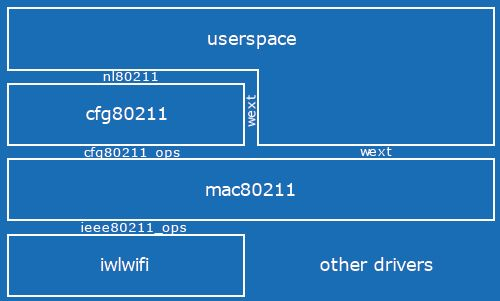
\includegraphics[width=0.8\hsize]{image201512/mac80211_arch.jpg}
\caption{nl80211の図示}
\end{figure}

\end{frame}


\begin{frame}{hostapdはどのようにWLI-UC-GNM2を操作するのか?(つづき)}

  cfg8011とhostapdは通信をしてWLI-UC-GNM2を操作するのですが、こちらで使われる
 プロトコルは、linuxのNETLINKが利用されます。

\end{frame}

  
\section{今後のイベント}
\emtext{今後のイベント}
\begin{frame}{今後のイベント}
\begin{itemize}
\item 関西エリアDebian勉強会。
\item 1/23(土) 14:00-19:00 第135回東京エリアDebian勉強会\\
  場所はdotsさんにて。
\end{itemize}
\end{frame}

\section{今日の宴会場所}
\emtext{今日の宴会場所}
\begin{frame}{今日の宴会場所}
未定
\end{frame}

\end{document}

;;; Local Variables: ***
;;; outline-regexp: "\\([ 	]*\\\\\\(documentstyle\\|documentclass\\|emtext\\|section\\|begin{frame}\\)\\*?[ 	]*[[{]\\|[]+\\)" ***
;;; End: ***
